\section{Streuungsmaße}
Um eine Verteilung sinnvoll beschreiben zu können sind zusätzlich zu den Lagemaßen noch Aussagen über die Streuung der Daten um das Mittel nötig.

\begin{definition}{Streuungsmaß}
	Ein \emph{Streuungsmaß} ist eine Abbildung $S:\R^n\rightarrow \R$ für die gilt
	\begin{equation*}
		S(x_1+a,\ldots,x_n+a)=S(x_1,\ldots,x_n) \quad\forall a,x_i\in\R (1\leq i\leq n)
	\end{equation*}
	Ein Streuungsmaß stellt dar, wie weit gestreut Werte einer Verteilung um ein Mittel liegen.
\end{definition}

\subsection{Variationsbreite, Stichprobenspannweite}
Die Stichproblenspannweite stellt dar, in welchem Bereich die Ausprägungen liegen, denn diese ist einfach
\begin{equation*}
	x_{\operatorname{max}}-x_{\operatorname{min}}.
\end{equation*}

\subsection{Standardabweichung}
Die Standardabweichung ist für eine Urliste $U=\simpleset{x_1,\ldots,x_n}$ von metrischen Daten definiert als
\begin{equation*}
	\tilde s=\sqrt{\frac 1n\sum_{i=1}^n (x_i-\overline x)^2}=\sqrt{\sum_{i=1}^n (a_i-\overline x)^2*f_i}
\end{equation*}
wobei die $a_i$ die Ausprägungen der Urliste sind und $f_i$ die relative Häufigkeit der Ausprägung $a_i$ ist.

Unter einer linearen Transformation $x\mapsto ax+b$ der Ausprägungen wird $\tilde s$ um $|a|$ gedehnt. Eine Verschiebung der Werte um $b$ hat keine Auswirkung.

\subsection{Variationskoeffizient}
Der Variationskoeffizient ist eine maßstabsunabhängige Maßzahl für die Streuung, sie basiert auf der Standardabweichung und ist definiert als
\begin{equation*}
	v=\frac{\tilde s}{\overline x},\quad \overline x>0
\end{equation*}

\subsection{Varianz, empirische Varianz}
Die empirische Varianz ist das Quadrat der Standardabweichung $\tilde s^2$.

\subsection{Stichprobenvarianz}
Die Stichprobenvarianz stellt ein nicht resistentes Streuungsmaß dar. Sie ist für eine Urliste $U=\simpleset{x_1,\ldots,x_n}$ definiert als
\begin{equation*}
	s^2=\frac{1}{n-1}\sum_{i=1}^n (x_i-\overline x)^2=\frac{1}{n-1}\sum_{i=1}^n x_i^2 - n*\overline x^2
\end{equation*}

\subsection{Mittlere absolute Abweichung vom Median}
Die mittlere absolute Abweichung vom Median stellt eine robustere Alternative zur Stichprobenvarianz dar. Sie ist für eine Urliste $U=\simpleset{x_1,\ldots,x_n}$ definiert als 
\begin{equation*}
	\frac 1n\sum_{i=1}^n|x_i-x_{\operatorname{med}}|
\end{equation*}


\subsection{Quantile}
Ein Quantil ist eine Kennzahl, die Daten nach einer relativen Häufigkeit trennt. So trennt das $p$-Quantil einer Verteilung die Daten som dass etwa $p*100\%$ der Daten darunter und $(1-p)*100\%$ darüber liegen. Damit ist der Median gerade das $50\%$-Quantil.

\begin{definition}{Quantile}
	Sei $U=\simpleset{x_1,\ldots,x_n}$ eine geordnete Urliste, d.h. $x_1\leq\ldots\leq x_j\leq\ldots\leq x_n$. Das $p$-Quantil $x_p$ ist eine Ausprägung $x_p\in U$ für die gilt
	\begin{equation*}
		\frac{\left|\set{i\in\N}{x_i\leq x_p, x_i\in U}\right|}{n}\geq p \text{ und } \frac{\left|\set{i\in\N}{x_i\geq x_p, x_i\in U}\right|}{n}\geq 1-p
	\end{equation*}
	Das heißt es liegen $p\%$ der Daten unterhalb und $(1-p)\%$ der Daten oberhalb des $p$-Quantils.

	Sinnvoll berechnen lässt sich das $p$-Quantil durch die Formel
	\begin{equation*}
		x_p=\begin{cases}
			\frac12(x_{(n*p)}+x_{(n*p+1)}) &\text{, falls $n*p$ ganzzahlig}\\
			x_{(\lfloor n*p\rfloor)+1} &\text{ sonst}
		\end{cases}
	\end{equation*}
\end{definition}
Dabei nennt man das $25\%$-Quantil auch das \emph{untere Quartil} und entsprechend das $75\%$-Quantil das \emph{obere Quartil}.

\begin{definition}{Interquartilsabstand}
	Für metrische Merkamel ist der sogenannte \emph{Interquartilsabstand (interquartile range)} die Distanz
	\begin{equation*}
		d_Q=\operatorname{IQR}=x_{0.75}-x_{0.25}.
	\end{equation*}
	Der IQR wird zum Beispiel beim Box-Plot verwendet. 
\end{definition}
Mit dem IQR können Zäune festgelegt werden, außerhalb derer sich höchstwahrscheinlich Ausreißer des Merkmals befinden. Ein Beispiel hierfür ist zum Beispiel der untere Zaun $z_u=x_{0.25}-1.5*d_Q$ und entsprechend die Obergrenze $z_o=x_{0.75}+1.5*d_q$, diese Werte werden wiederum beim Box-Plot verwendet.

\subsubsection{Box-Plot}
Das Box-Plot ist eine einfache Art und Weise die Ausprägungen einer Verteilung übersichtlich darzustellen. Für den Box-Plot ist ein 5-Tupel, $(z_u, x_{0.25}, x_{\operatorname{med}}, x_{0.75}, z_o)$ aus Werten ausreichend.
Beim Boxplot werden zwei Definitionen unterschieden, der \glqq normale\grqq\ Box-Plot und der modifizierte.

Beim Box-Plot wird ein Rechteck zwischen $x_{0.25}$ und $x_{0.75}$ gezeichnet, das $x_{\operatorname{med}}$ beinhaltet.
So sieht man dass sich 50\% der Datenpunkte innerhalb der Box befinden. Die nach außen gezeichneten Linien geben an, wie weit die Datenpunkte gestreut liegen. Diese sogenannten Whiskers enden bei $z_u$ bzw. $z_o$, diese Werte unterscheiden sich bei den beiden Definitionen.

\paragraph{Normaler Box-Plot}
Das Fünftupel besteht aus den Werten $(x_{\operatorname{min}}, x_{0.25}, x_{\operatorname{med}}, x_{0.75}, x_{\operatorname{max}})$. Wobei $x_{\operatorname{min}}$ und $x_{\operatorname{max}}$ die kleinste und größte Ausprägung der Verteilung darstellen. So sind alle Werte in der Spannweite der Whiskers enthalten. Ein Box-Plot sieht dann wie folgt aus

\begin{center}
	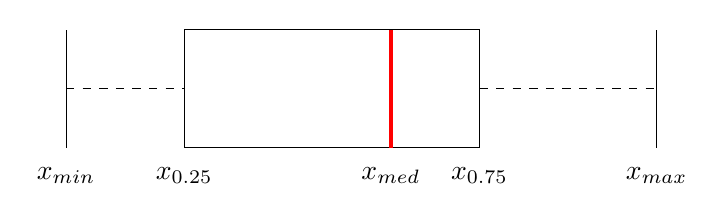
\begin{tikzpicture}[scale=0.75]
		\draw[black] (0,0) rectangle (5,2);
		\draw[black, dashed] (-2, 1) to (0,1) (5,1) to (8,1);
		\draw[black] (-2,0) to (-2,2) (8,0) to (8,2);
		\draw[red, line width=0.5mm] (3.5,0) to (3.5,2);

		\draw (-2,0) node[label={below:$x_{\operatorname{min}}$}] {};
		\draw (0,0) node[label={below:$x_{0.25}$}] {};
		\draw (3.5,0) node[label={below:$x_{\operatorname{med}}$}] {};
		\draw (5,0) node[label={below:$x_{0.75}$}] {};
		\draw (8,0) node[label={below:$x_{\operatorname{max}}$}] {};
	\end{tikzpicture}
\end{center}


\paragraph{Modifizierter Box-Plot (nach Fahrmeir)}
Der wichtigste Unterschied zum normalen Box-Plot ist dass, anstatt der minimalen und maximalen Werte für $z_u, z_o$ ein Zaun gewählt wurde. So ist $z_u=x_{0.25}-1.5*d_Q$ und $z_o=x_{0.75}+1.5*d_Q$ wobei $d_Q$ der Interquartilsabstand ist. Allerdings ist zu beachten dass die Whiskers von der größten/ kleinsten Ausprägung innerhalb des Zauns zur Box ausgehen. Liegen also beispielweise innerhalb des Bereichs $[z_u,x_{0.25}]$ keine Datenwerte, so existiert kein unterer Whisker. Datenpunkte, die außerhalb des Zauns liegen, werden mit Punkten dargestellt. Dies ist ein gutes Anzeichen für eventuelle Ausreißer.

\begin{center}
	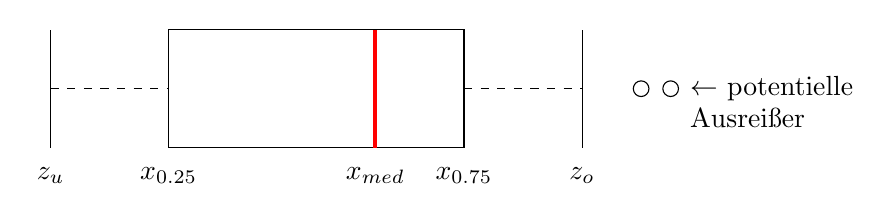
\begin{tikzpicture}[scale=0.75]
		\draw[black] (0,0) rectangle (5,2);
		\draw[black, dashed] (-2, 1) to (0,1) (5,1) to (7,1);
		\draw[black] (-2,0) to (-2,2) (7,0) to (7,2);
		\draw[red, line width=0.5mm] (3.5,0) to (3.5,2);

		\draw (-2,0) node[label={below:$z_u$}] {};
		\draw (0,0) node[label={below:$x_{0.25}$}] {};
		\draw (3.5,0) node[label={below:$x_{\operatorname{med}}$}] {};
		\draw (5,0) node[label={below:$x_{0.75}$}] {};
		\draw (7,0) node[label={below:$z_o$}] {};
		\draw (8,1) node[draw=black, fill=white, circle, inner sep=2pt] {};
		\draw (8.5,1) node[draw=black, fill=white, circle, inner sep=2pt] {};
		\draw (8.5,1) node[label={right:$\leftarrow$\ potentielle}] {};
		\draw (8.5,0.5) node[label={right:Ausreißer}] {};
	\end{tikzpicture}
\end{center}


